\begin{figure}
    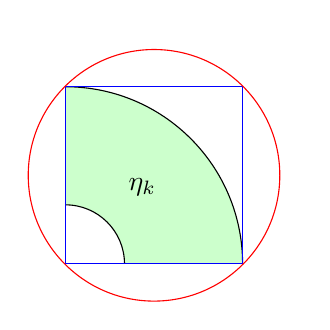
\begin{tikzpicture}[scale=0.75]
      \begin{scope}
        \clip (0,0) rectangle (4,4);
        \draw[fill=green!20] (0,0) circle (3cm);
        \draw[fill=white] (0,0) circle (1cm);  
      \end{scope}
      \draw[blue] (0,0) -- (3,0) -- (3,3) -- (0,3) -- (0,0);
      \draw[red]  (1.5,1.5) circle (2.13cm);
      \node at (1.3,1.3) {$\eta_k$};    
    \end{tikzpicture} 
    \caption{\scriptsize{An \emph{I-state} $\eta_k$ (shaded region),
        over-approximations $A(\eta_k)$ using disk (red circle) and rectangle
        (blue). }}
\end{figure}